% Panel (b) of pub_rse_methodology/goldstandard_empirical.tex: the RIGHT cascade
% annotated with the DELFI corpus (n = 266). Panel (a) is dropped here because
% the normative model gets its own slide (fig-right.pdf).
\documentclass[tikz,border=6pt]{standalone}
% Shared preamble for the standalone renders of the RIGHT-framework figures.
% The tikz styles are copied verbatim from pub_rse_methodology/uml_shapes.tex so
% that the standalone PDFs look exactly like the ones in the paper.
\usepackage[utf8]{inputenc}
\usepackage[T1]{fontenc}
\usepackage{graphicx}
\usepackage{times}
\usepackage{amssymb}
\usepackage{xcolor}
\usepackage{tikz}
\usetikzlibrary{arrows.meta,positioning,shapes.geometric,shapes.misc,calc}

\tikzset {
    initial/.style={circle, fill=black, minimum size=5mm, inner sep=0pt},
    action/.style={draw, rounded corners=2pt, minimum width=28mm,
        minimum height=8mm, align=center},
    decision/.style={draw, diamond, aspect=2, minimum height=8mm,
        minimum width=8mm, inner sep=1pt, align=center},
    fork/.style={draw, fill=black, minimum width=20mm, minimum height=4mm},
    vfork/.style={draw, fill=black, minimum width=2mm, minimum height=14mm},
    box/.style={draw, rounded corners=2mm, thick, minimum width=18mm,
        minimum height=8mm, align=center},
    rsepic/.style={inner sep=0pt, outer sep=2pt},
    dependency/.style={dashed, <->},
    node distance=8mm,
    uml_activity/.style={draw, line width=0.6pt,
        -{Straight Barb[angle=40:5pt 5]}},
    >=Latex,
    every path/.style={uml_activity}
}

\newcommand{\terminus}{
\includegraphics[height=6mm]{uml_endnode.png}}
\newcommand{\rsecycle}{
\includegraphics[height=12mm]{rse-cycle.png}}


\definecolor{decfill}{HTML}{DCE8F5}
\definecolor{metfill}{HTML}{DCF0DC}
\definecolor{usedcol}{HTML}{333333}
\definecolor{shouldcol}{HTML}{1F5FA8}
\definecolor{nocol}{HTML}{C0392B}
\definecolor{yescol}{HTML}{1F5FA8}
\providecommand{\usel}{\scriptsize\color{usedcol}}
\providecommand{\shdl}{\scriptsize\color{shouldcol}}

\begin{document}
    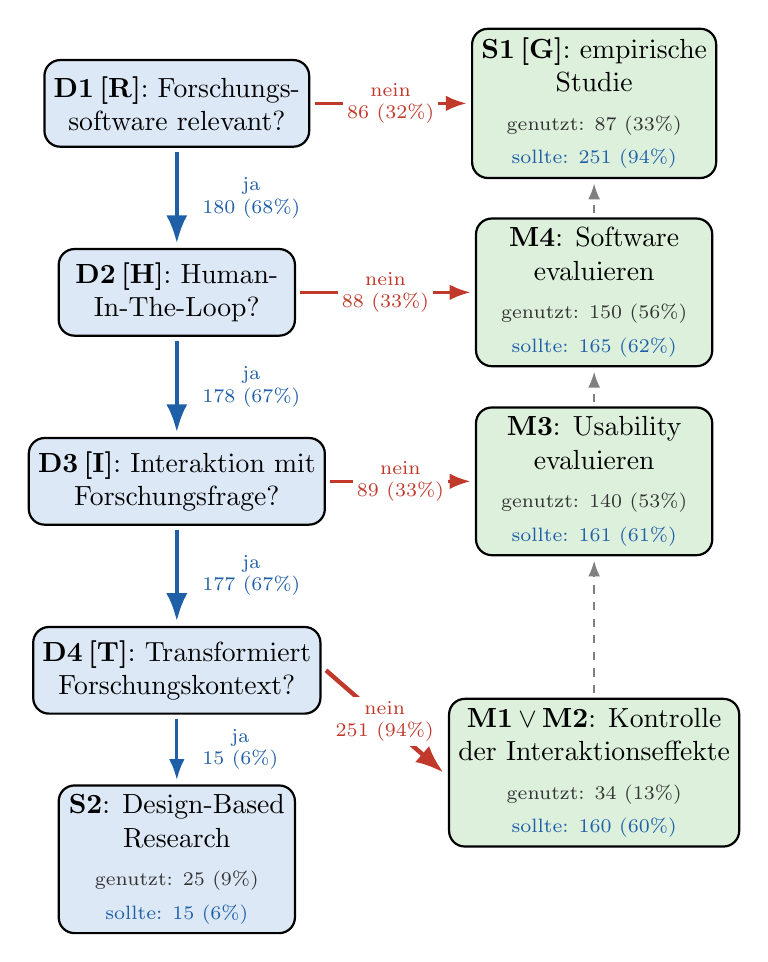
\begin{tikzpicture}[
        >=Latex,
        every node/.style={outer sep=2pt},
        dbox/.style={draw, rounded corners=2mm, thick, fill=decfill,
            minimum width=30mm, minimum height=11mm, align=center},
        mbox/.style={draw, rounded corners=2mm, thick, fill=metfill,
            minimum width=30mm, minimum height=13mm, align=center},
        elab/.style={font=\scriptsize, align=center, fill=white, inner sep=1.5pt},
    ]

    \node[dbox] at ( 0, 0)   (b1) {\textbf{D1\,[R]}: Forschungs-\\software relevant?};
    \node[dbox] at ( 0,-2.4) (b2) {\textbf{D2\,[H]}: Human-\\In-The-Loop?};
    \node[dbox] at ( 0,-4.8) (b3) {\textbf{D3\,[I]}: Interaktion mit\\Forschungsfrage?};
    \node[dbox] at ( 0,-7.2) (b4) {\textbf{D4\,[T]}: Transformiert\\Forschungskontext?};
    \node[dbox] at ( 0,-9.6) (bs2) {\textbf{S2}: Design-Based\\Research\\[2pt]
        {\usel genutzt: 25 (9\%)}\\{\shdl sollte: 15 (6\%)}};

    \node[mbox] at ( 5.3, 0)   (bs1) {\textbf{S1\,[G]}: empirische\\Studie\\[2pt]
        {\usel genutzt: 87 (33\%)}\\{\shdl sollte: 251 (94\%)}};
    \node[mbox] at ( 5.3,-2.4) (bm4) {\textbf{M4}: Software\\evaluieren\\[2pt]
        {\usel genutzt: 150 (56\%)}\\{\shdl sollte: 165 (62\%)}};
    \node[mbox] at ( 5.3,-4.8) (bm3) {\textbf{M3}: Usability\\evaluieren\\[2pt]
        {\usel genutzt: 140 (53\%)}\\{\shdl sollte: 161 (61\%)}};
    \node[mbox, yshift=-1.3cm] at ( 5.3,-7.2) (bm1) {\textbf{M1\,$\vee$\,M2}: Kontrolle\\der Interaktionseffekte\\[2pt]
        {\usel genutzt: 34 (13\%)}\\{\shdl sollte: 160 (60\%)}};

    \draw[->, line width=1.0pt, nocol] (b1.east) --
        node[elab, midway, text=nocol]{nein\\86 (32\%)} (bs1.west);
    \draw[->, line width=1.0pt, nocol] (b2.east) --
        node[elab, midway, text=nocol]{nein\\88 (33\%)} (bm4.west);
    \draw[->, line width=1.0pt, nocol] (b3.east) --
        node[elab, midway, text=nocol]{nein\\89 (33\%)} (bm3.west);
    \draw[->, line width=1.6pt, nocol] (b4.east) --
        node[elab, pos=0.5, text=nocol]{nein\\251 (94\%)} (bm1.west);

    \draw[->, line width=1.6pt, yescol] (b1.south) --
        node[elab, midway, right, xshift=2mm, text=yescol]{ja\\180 (68\%)} (b2.north);
    \draw[->, line width=1.6pt, yescol] (b2.south) --
        node[elab, midway, right, xshift=2mm, text=yescol]{ja\\178 (67\%)} (b3.north);
    \draw[->, line width=1.6pt, yescol] (b3.south) --
        node[elab, midway, right, xshift=2mm, text=yescol]{ja\\177 (67\%)} (b4.north);
    \draw[->, line width=1.0pt, yescol] (b4.south) --
        node[elab, midway, right, xshift=2mm, text=yescol]{ja\\15 (6\%)} (bs2.north);

    \draw[->, dashed, gray] (bm4.north) -- (bs1.south);
    \draw[->, dashed, gray] (bm3.north) -- (bm4.south);
    \draw[->, dashed, gray] (bm1.north) -- (bm3.south);

    \end{tikzpicture}
\end{document}
